% !TeX spellcheck = it_IT

\chapter{MPI}\label{sec:second_mpi}
\emph{MPI} cioè, Message Passing Interface, è uno \textit{standard per l'interfaccia di una libreria per lo scambio di messaggi} \cite{mpi_standard}.\\
Questo standard \textit{de facto} è nato grazie al lavoro svolto su \textit{MPI Forum}, un forum nel quale aziende che si occupano di \textquotedblleft Parallel Computing\textquotedblright, ricercatori nell'ambito informatico, sviluppatori di librerie e di applicazioni hanno collaborato per raggiungere questo risultato.\\
Come detto \textit{MPI} è una specifica e non una libreria e si propone quindi di imporre regole e di dare istruzioni su quello che una libreria per lo scambio di messaggi deve fare. Inoltre, non essendo \textit{MPI} un linguaggio di programmazione tutte le operazioni sono espresse come funzioni, subroutine, o metodi a seconda del \textit{binding} con i linguaggi che fanno parte dello standard.\\
L'obbiettivo di \textit{MPI}, quindi, è quello di stabilire uno standard per il \textit{message-passing} \emph{portabile}, \emph{flessibile}, \emph{pratico} ed \emph{efficiente}.\\
\textit{MPI} è rivolto principalmente al modello di \textit{message-passing} nella \textit{programmazione parallela}, in cui i dati vengono spostati dallo spazio di indirizzi di un processo a quello di un altro tramite operazioni cooperative su ciascun processo.\\
In particolare in un ambiente di comunicazione a memoria distribuita, in cui le astrazioni di livello superiore sono costruite sulla base del livello inferiore, ovvero sulle routine di \textit{message-passing}, i benefici della standardizzazione sono particolarmente evidenti.\\
Inoltre, la definizione di uno standard \textit{message-passing}, come quella proposta da MPI, fornisce un insieme di funzioni base ben definito, efficientemente implementabili dai vendor interessati al \textquotedblleft Parallel Computing\textquotedblright, o per le quali sia possibile fornire supporto hardware, rafforzando in tal modo la scalabilità.\\
L'obiettivo di \textit{MPI} è quindi quello di sviluppare uno standard ampiamente utilizzato per la scrittura di programmi di \textit{message-passing}.

\subsection{La struttura di un programma MPI}
Un programma \textit{MPI} è un programma che, seguendo le procedure introdotte dallo standard, esegue operazioni di \textit{message-passing} su architetture di calcolo parallelo.\\
D'ora in avanti si affronteranno programmi \textit{MPI} in \textit{C/C++} che utilizzano la libreria \emph{OpenMPI} \cite{open_mpi} per l'implementazione delle funzioni, ma le considerazioni fatte sono comunque valide per le relative funzioni legate al \textit{Fortran} e per implementazioni di altre librerie.\\
Ogni programma \textit{MPI} deve utilizzare la direttiva del preprocessore: \lstinline{#include "mpi.h"}\\
\textit{mpi.h} infatti contiene le definizioni, le macro e i prototipi delle funzioni necessari per compilare un programma \textit{MPI}.\\
Prima di ogni altra funzione \textit{MPI} bisogna invocare la funzione \textit{MPI\_Init()}; questa funzione deve essere chiamata una sola volta. La \textit{MPI\_Init()} prende come argomenti i puntatori ai parametri del \textit{main} e permette al sistema di preparare l'ambiente per l'esecuzione delle varie routine \textit{MPI} che possono essere usate.\\
Una volta che il programma ha finito di utilizzare le funzioni \textit{MPI} deve chiamare la \textit{MPI\_Finalize()} che permette di \textquotedblleft pulire\textquotedblright~ogni lavoro non terminato dalle varie funzioni \textit{MPI} invocate precedentemente.\\
Nel listato \ref{lst:genic_mpi} è mostrata la generica struttura di un programma \textit{MPI} \cite{mpi_general}.\\
\begin{lstlisting}[label={lst:genic_mpi},
caption={Programma MPI generico}]

(*@~ ~ ~ ~\raisebox{-1pt}[0pt][0pt]{$\vdots$}@*)

#include (*@\textquotedblleft@*)mpi.h"

(*@~ ~ ~ ~\raisebox{-1pt}[0pt][0pt]{$\vdots$}@*)

main(int argc, char** argv){

(*@~ ~ ~ ~ ~ ~ ~ ~ ~ ~{\raisebox{-1pt}[0pt][0pt]{$\vdots$}}@*)

    //Nessuna chiamata a funzioni MPI prima di questa
    MPI_Init(&argc, &argv);

(*@~ ~ ~ ~ ~ ~ ~ ~ ~ ~{\raisebox{-1pt}[0pt][0pt]{$\vdots$}}@*)

    MPI_Finalize();
    //Nessuna chiamata a funzioni MPI dopo questa

(*@~ ~ ~ ~ ~ ~ ~ ~ ~ ~{\raisebox{-1pt}[0pt][0pt]{$\vdots$}}@*)
}

\end{lstlisting}
\subsection{Le principali componenti}\label{subsec:comm_mpi}
In MPI la comunicazione fra i processi si basa sullo scambio di messaggi.\\
MPI quindi definisce le strutture e le informazioni che servono per realizzare uno scambio di messaggi tra processi.\\
In particolare lo standard descrive:
\begin{itemize}
	\item In che modo rappresentare il dato, da inviare nel messaggio, durante la comunicazione;
	\item Come specificare i processi protagonisti dello scambio del messaggio;
	\item I vari modi in cui può essere implementata la comunicazione.
\end{itemize}  
\subsubsection{Definizione dei dati in MPI}\label{subsec:def_dati_mpi}
Per poter inviare un dato attraverso un messaggio, che poi verrà scambiato tra i processi, occorre definire alcune informazioni fondamentali legate al dato stesso; in particolare è necessario definire:
\begin{itemize}
	\item \textbf{Il buffer}, ovvero l'indirizzo di memoria che contiene i dati da inviare;
	\item \textbf{Il numero di elementi} da inviare nel messaggio;
	\item \textbf{Il tipo di dato} degli elementi.
\end{itemize}
Il tipo di dato può rispecchiare uno dei tipi di dato più comuni del linguaggio \textit{C} (figura \ref{fig:mpi_data_types}) oppure può essere un tipo di dato definito da utente in quanto MPI fornisce le primitive per costruire strutture dati partendo da altre già esistenti.
\begin{figure}[H]
	\centering
	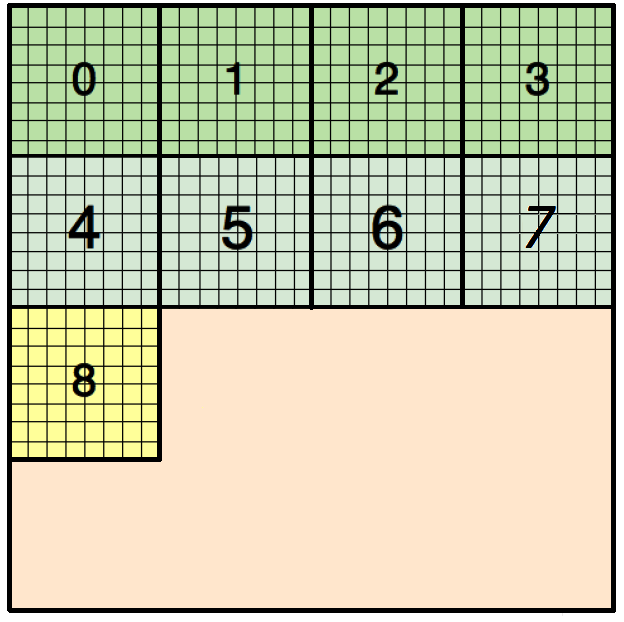
\includegraphics[width=0.6\textwidth]{immagini/block_on_grid.png}
	\caption{Tipi di dato in C e in MPI}
	\label{fig:mpi_data_types}
\end{figure}
\subsubsection{Specificazione dei processi coinvolti nella comunicazione}\label{subsec:comm_rank_tag}
Durante l'invio di un messaggio è necessario specificare il destinatario e garantire che le informazioni che lo identificano siano univoche per non compromettere la comunicazione.\\
A questo scopo durante l'invio di un messaggio MPI bisogna sempre indicare:
\begin{itemize}
	\item \textbf{Il communicator} che rappresenta uno specifico contesto a cui appartiene un gruppo di processi (il \textit{communicator} di default si chiama \textit{MPI\_COMM\_WORLD} e racchiude tutti i processi disponibili).
	\begin{figure}[H]
		\centering
		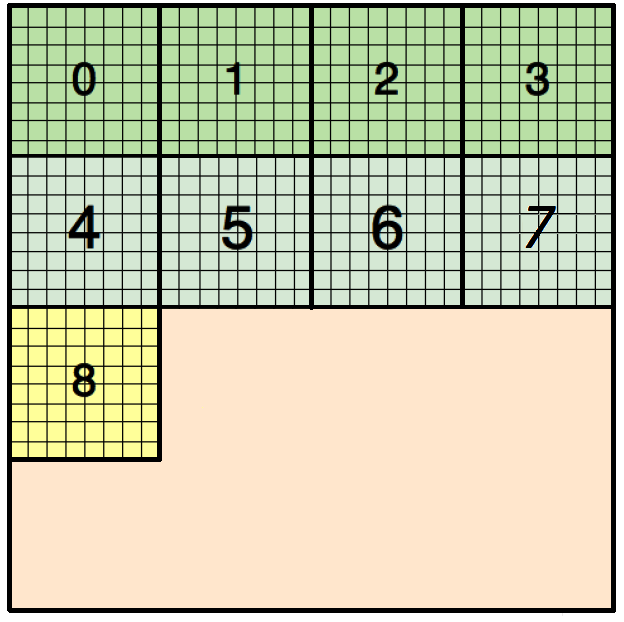
\includegraphics[width=0.5\textwidth]{immagini/block_on_grid.png}
		\caption{Il \textit{communicator MPI\_COMM\_WORLD} e due sottogruppi}
		\label{fig:mpi_communicator}
	\end{figure}
	\item \textbf{Il rank}, che è un identificativo univoco assegnato ad ogni processo, del processo destinatario;
	\item \textbf{Il tag} che permette, grazie ad un intero definito da utente, di differenziare ulteriormente il messaggio.
\end{itemize}

\subsubsection{Le implementazioni delle comunicazioni punto a punto}
MPI prevede diverse modalità per gestire la comunicazione tra i processi.
\paragraph{La comunicazione standard}~\newline~\newline
La modalità standard è \emph{bloccante e asincrona} si effettua utilizzando la funzioni \textit{MPI\_Send} per l'invio e \textit{MPI\_Recv} per la ricezione.\\
\begin{lstlisting}[label={lst:mpi_send_recv},
caption={Intestazioni delle primitive di comunicazione MPI}]
MPI_Send(void *buf, int count, MPI_Datatype datatype, int dest, int tag, MPI_Comm comm)
         
MPI_Recv(void *buf, int count, MPI_Datatype datatype, int source, int tag, MPI_Comm comm, MPI_Status *status)
\end{lstlisting}

In entrambe le funzioni i parametri \textit{buf}, \textit{count} e \textit{datatype} servono per fornire le informazioni sul contenuto nel messaggio come spiegato nel paragrafo \ref{subsec:def_dati_mpi}.\\
Il parametro \textit{dest} nella funzione di invio e il parametro \textit{source} in quella di ricezione indicano rispettivamente il \textit{rank} del processo che deve ricevere e di quello che deve inviare i dati. Oltre al \textit{rank} dei processi coinvolti, queste funzioni prendono in argomento anche le altre informazioni illustrate nel paragrafo \ref{subsec:comm_rank_tag} relative al destinatario; in particolare richiedono: il \textit{tag} del messaggio e il \textit{communicator(comm)} nel quale si svolge la comunicazione.\\
La funzione \textit{MPI\_Recv} grazie a \textit{status} può ottenere informazioni aggiuntive sul messaggio.\\
Essendo la \textit{MPI\_Send} bloccante, ritorna solo quando i dati sono stati copiati nel buffer di sistema del destinatario e quindi, per esempio, se il buffer è pieno, la funzione resta bloccata in attesa che si liberi. Una volta che la funzione è ritornata, non c’è alcuna garanzia che il processo destinatario abbia ricevuto il messaggio.\\
A sua volta la \textit{MPI\_Recv}, essendo bloccante ritorna solamente quando i dati sono stati copiati dal buffer di sistema all’indirizzo di memoria specificato.\\
Lo schema di una comunicazione bloccante è mostrato in figura \ref{fig:mpi_block_com}.
\begin{figure}[H]
	\centering
	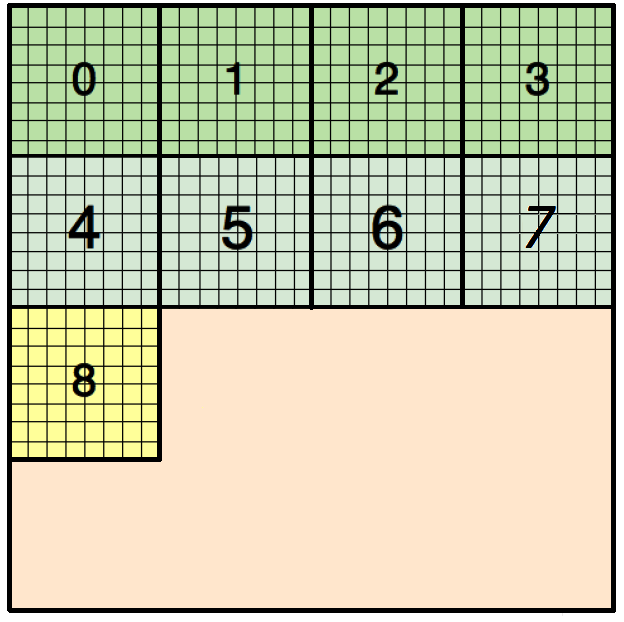
\includegraphics[width=0.7\textwidth]{immagini/block_on_grid.png}
	\caption{Schema di una comunicazione bloccante}
	\label{fig:mpi_block_com}
\end{figure}
\paragraph{Altri tipi di comunicazione punto a punto}~\newline~\newline
Oltre alla modalità standard (asincrona) MPI definisce altre modalità, \textit{bloccanti e non}, di comunicazione per l’invio di un messaggio.\\
Le seguenti modalità di invio sono \emph{bloccanti} e richiedono come parametri gli stessi richiesti dalla funzione primitiva MPI\_Send:
\begin{itemize}
	\item MPI\_Ssend ($\cdots$): questa funzione ritorna solo quando il destinatario ha iniziato a ricevere;
	\item MPI\_Bsend ($\cdots$): questa funzione ritorna quando i dati sono copiati in un buffer specifico;
	\item MPI\_Rsend ($\cdots$): da utilizzare solo quando si è certi che il destinatario sia in ascolto.
\end{itemize}
Esistono anche modalità di comunicazione \emph{non bloccanti} (di cui viene mostrato lo schema in figura \ref{fig:mpi_non_block_comm}) che vengono descritte dalle seguenti funzioni nel codice \ref{lst:mpi_send_recv_non_blocc}.\\
\begin{lstlisting}[ 
label={lst:mpi_send_recv_non_blocc},
caption={Intestazioni delle comunicazioni non bloccanti MPI}]
MPI_Isend(void* buf, int count, MPI_Datatype datatype, int dest, int tag, MPI_Comm comm, MPI_Request &request)

MPI_Irecv(void* buf, int count, MPI_Datatype datatype, int source, int tag, MPI_Comm comm, MPI_Request &request)
\end{lstlisting}
Le funzioni sopracitate ritornano immediatamente, ma la memoria all’indirizzo \textit{buf} non può essere scritta o letta finché non si è certi della conclusione dell’operazione.\\
Il campo \textit{request} delle due funzioni è un \textit{handle} che permette di verificare e interagire con lo status della richiesta grazie ad opportune funzioni (MPI\_Test e MPI\_Wait).
\begin{figure}[H]
	\centering
	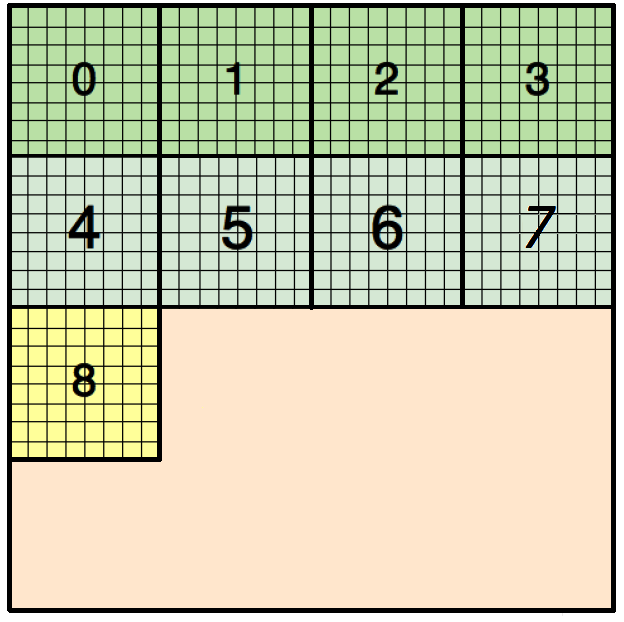
\includegraphics[width=0.7\textwidth]{immagini/block_on_grid.png}
	\caption{Schema di una comunicazione non bloccante}
	\label{fig:mpi_non_block_comm}
\end{figure}
\subsubsection{Le comunicazioni collettive}\label{subsubsec:coll_comm}
Un ultimo tipo di comunicazione messo a disposizione da MPI è la comunicazione collettiva. Una comunicazione collettiva è una comunicazione che riguarda tutti i processi presenti all'interno di uno stesso \textit{communicator} che non interferisce con le comunicazioni \emph{punto-punto} e che non può essere bloccante.\\
MPI mette a disposizione diverse funzioni per gestire vari tipi di comunicazione collettiva (figura \ref{fig:mpi_collect_comm}):
\begin{itemize}
\item \textbf{MPI\_Bcast} per permettere ad un processo di inviare lo stesso messaggio a tutti gli altri;
\item \textbf{MPI\_Reduce} per permettere ad un processo di suddividere un messaggio tra tutti gli altri;
\item \textbf{MPI\_Scatter} per far si che tutti i processi inviino un messaggio ad uno stesso nodo;
\item \textbf{MPI\_Gather} per far si che tutti i processi cooperino per calcolare un risultato da inviare ad uno stesso processo.
\end{itemize}
\begin{figure}[H]
\centering
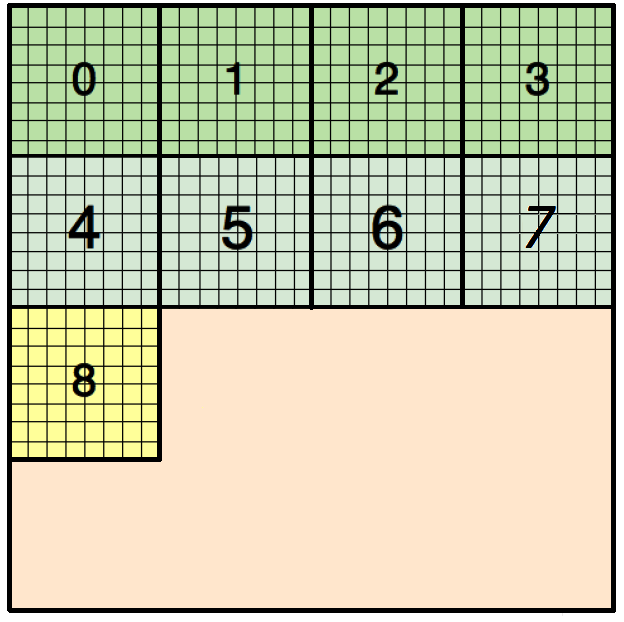
\includegraphics[width=0.55\textwidth]{immagini/block_on_grid.png}
\caption{Rappresentazione di alcune comunicazioni collettive}
\label{fig:mpi_collect_comm}
\end{figure}

\subsection{Il modello hardware per un ambiente MPI}\label{subsubsec:mpi_hw_model}
Come detto MPI è un'interfaccia per le librerie che si devono occupare di message-passing.\\
Questo scambio di informazioni è dunque legato ad un ambiente di calcolo parallelo e a una relativa architettura hardware che consente di eseguire uno stesso programma parallelamente su più processori o addirittura su più nodi.\\
Le varie configurazioni che può avere un ambiente di calcolo parallelo, secondo la tassonomia di Flynn (1986), derivano dalla configurazione hardware e software di due componenti principali del sistema: il \emph{flusso di istruzioni (processi)} e il \emph{flusso di dati}. Le varie configurazioni previste da questa suddivisione sono:
\begin{itemize}
	\item \textbf{SISD} (\textit{Single Instruction Single Data}): Architetture dei sistemi seriali, senza quindi, nessun grado di parallelismo (schema in figura \ref{fig:sisd});
	\item \textbf{SIMD} (\textit{Single Instruction Multiple Data}): Architetture composte da molte unità di elaborazione che eseguono contemporaneamente la stessa istruzione ma lavorano su insiemi di dati diversi (schema in figura \ref{fig:simd});
	\item \textbf{MISD} (\textit{Multiple Instruction Single Data}): Architetture in cui più flussi di istruzioni lavorano contemporaneamente su un unico flusso di dati (schema in figura \ref{fig:misd}). Questa tipologia di architettura non è stata praticamente mai adottata;
	\item \textbf{MIMD} (\textit{Multiple Instruction Multiple Data}): Architetture in cui più istruzioni vengono eseguite contemporaneamente su più dati diversi (schema in figura \ref{fig:mimd}). Sotto questa classificazione ricadono i \textit{cluster} di computer e di conseguenza l'ambiente sul quale è stato basato lo sviluppo di questa tesi.
\end{itemize}

\begin{figure}[H]
	\centering
	\begin{subfigure}{.5\textwidth}
		\centering
		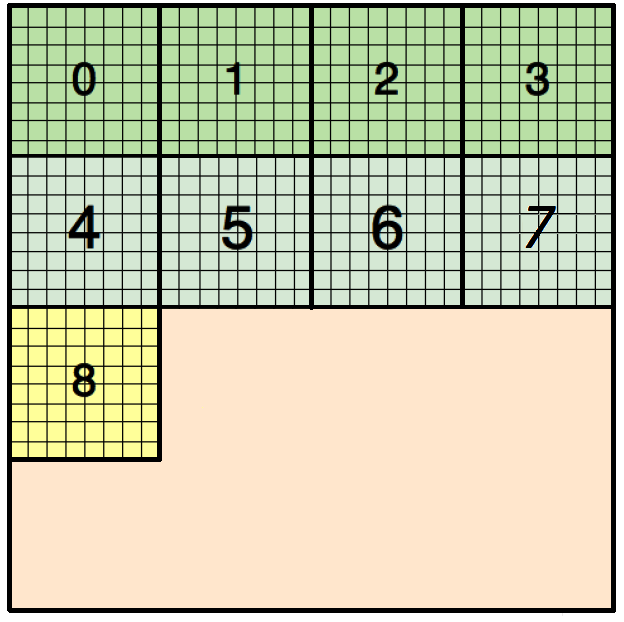
\includegraphics[width=0.45\linewidth]{immagini/block_on_grid.png}
		\caption{Architettura SISD\newline}
		\label{fig:sisd}
	\end{subfigure}%
	\begin{subfigure}{.5\textwidth}
		\centering
		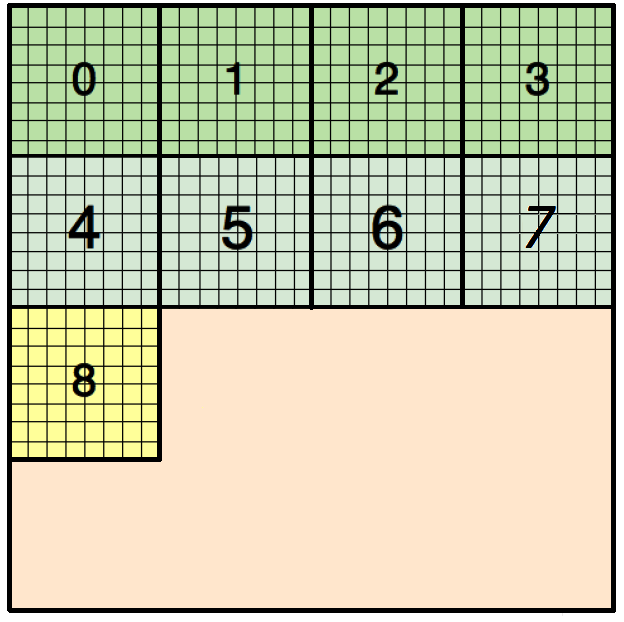
\includegraphics[width=0.45\linewidth]{immagini/block_on_grid.png}
		\caption{Architettura MISD\newline}
		\label{fig:misd}
	\end{subfigure}
	\label{fig:test}
	\begin{subfigure}{.5\textwidth}
		\centering
		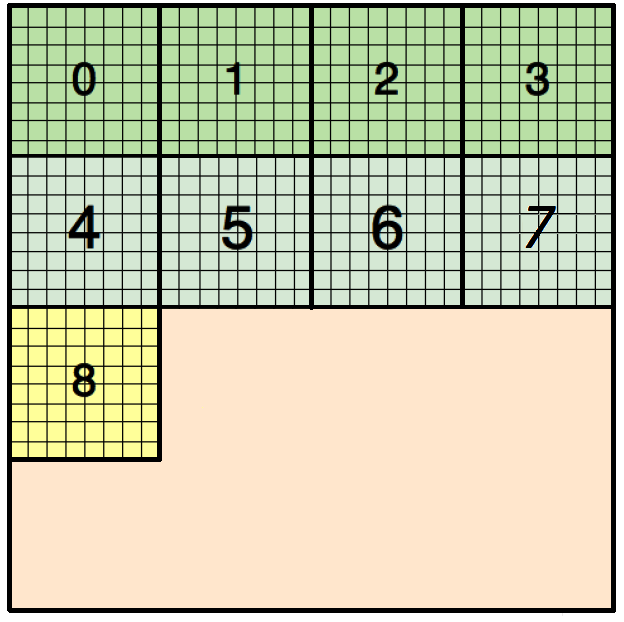
\includegraphics[width=0.45\linewidth]{immagini/block_on_grid.png}
		\caption{Architettura SIMD\newline}
		\label{fig:simd}
	\end{subfigure}%
	\begin{subfigure}{.5\textwidth}
		\centering
		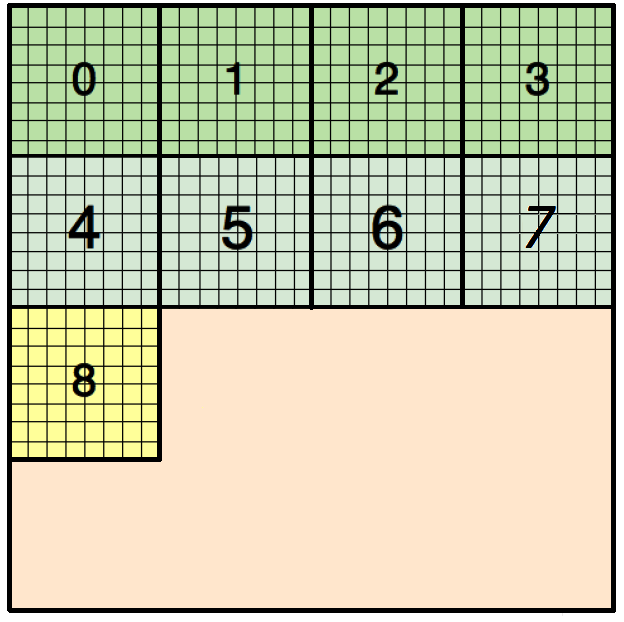
\includegraphics[width=0.45\linewidth]{immagini/block_on_grid.png}
		\caption{Architettura MIMD\newline}
		\label{fig:mimd}
	\end{subfigure}
	\caption{Le varie architetture della Tassonomia di Flynn}
\end{figure}

In particolare tra i sistemi MIMD possono distinguersi le architetture a \emph{memoria condivisa} (figura \ref{fig:mem_dist}) o quelle a \emph{memoria distribuita} (figura \ref{fig:mem_cond}).\\
Nella prima configurazione la memoria è condivisa fisicamente (UMA) o solo logicamente assegnando indirizzi globali alle vari memorie locali (NUMA), permettendo ai vari nodi di lavorare sugli stessi spazi di memoria, evitando quindi di dover gestire le comunicazioni.\\
Nell'architettura a memoria distribuita, ogni nodo possiede una propria memoria locale che non fa parte dello spazio di indirizzamento degli altri processori e, per regolare l'accesso di un nodo alle risorse che non sono locali, bisogna utilizzare protocolli di comunicazione e scambio dati come, per esempio, quelli descritti da MPI.
\begin{figure}[H]
	\centering
	\begin{subfigure}{0.5\textwidth}
		\centering
		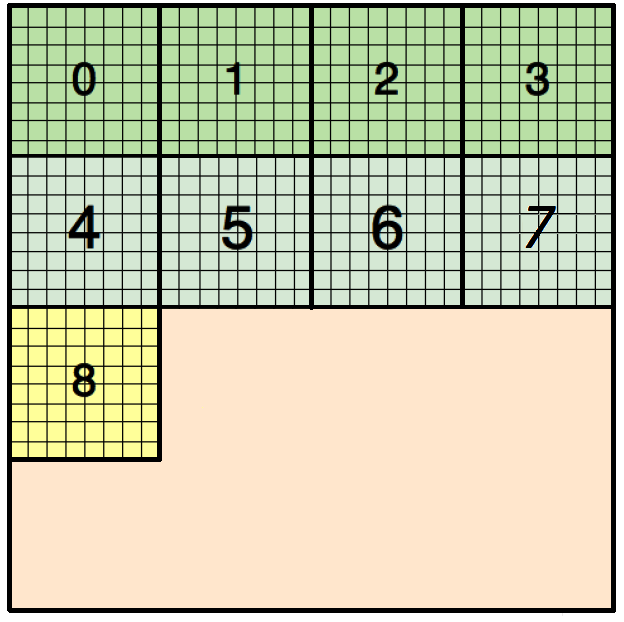
\includegraphics[width=0.9\linewidth]{immagini/block_on_grid.png}
		\caption{Memoria condivisa}
		\label{fig:mem_cond}
	\end{subfigure}%
	\begin{subfigure}{0.5\textwidth}
		\centering
		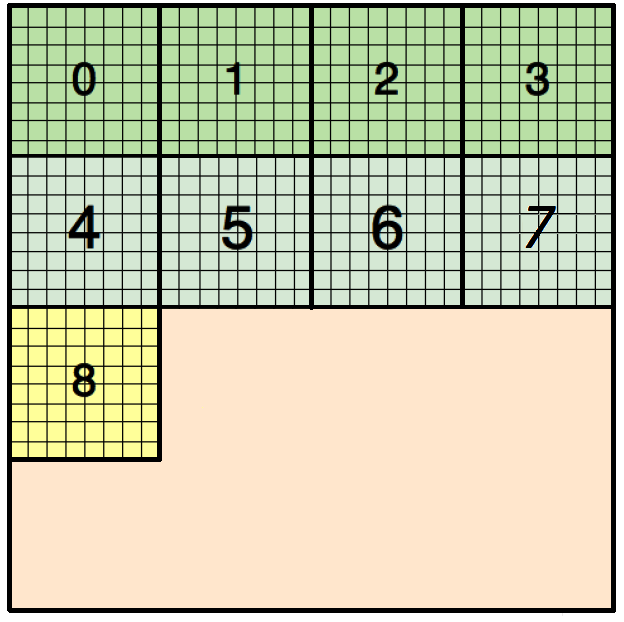
\includegraphics[width=1.0\linewidth]{immagini/block_on_grid.png}
		\caption{Memoria distribuita}
		\label{fig:mem_dist}
	\end{subfigure}
	\label{fig:mem_cond_dist}
	\caption{Le due diverse architetture MIMD}
\end{figure}
